{\setbeamerfont{framesubtitle}{size=\tiny}
\begin{frame}{\fe{Exercice 2 : fissuration par suppression d'éléments}
                 {Exercise 2: fracture by elements removal}}
             {\url{https://www-cast3m.cea.fr/index.php?page=exemples&exemple=formation_pasapas_2_initial}}
  \small
  \begin{itemize}
    \item \fe{Éprouvette entaillée en traction uniaxiale \textcolor{green}{(déplacements imposés)}}
             {Notched specimen in uniaxial tension \textcolor{green}{(imposed displacements)}}\\
    \hspace{1cm}
    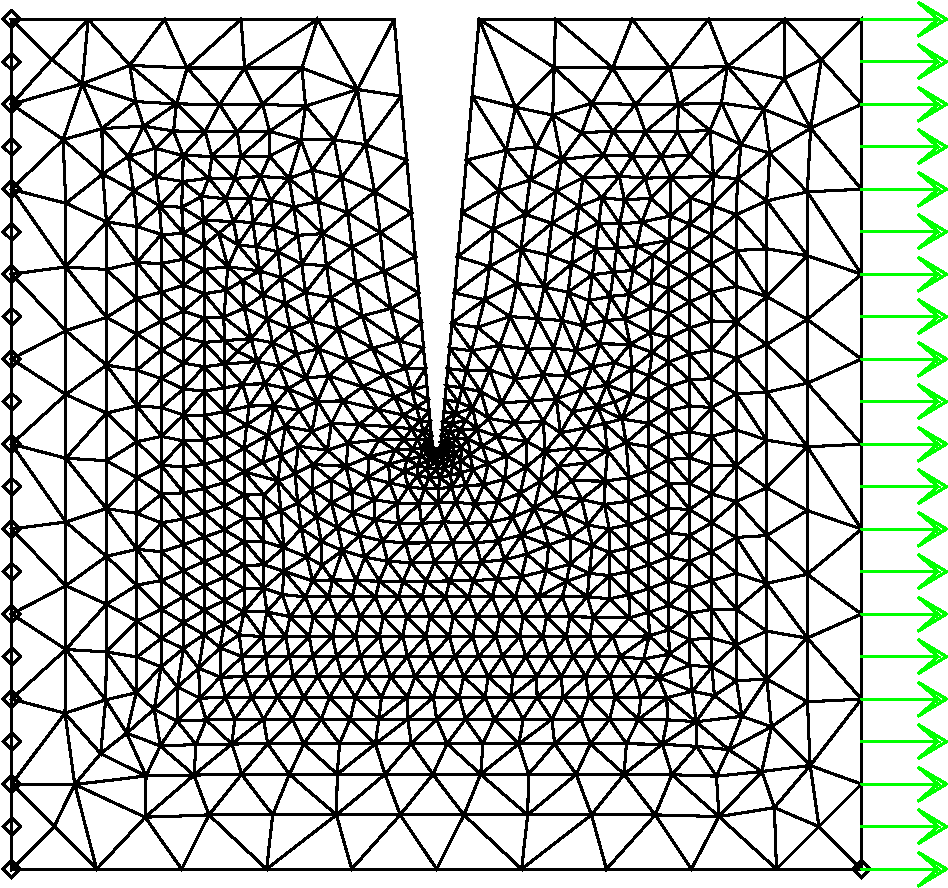
\includegraphics[height=3cm]{images/exo/exo_2_chargement} \hspace{0.2cm}
    \hspace{0.6cm}
    \if \animation 1
      \animategraphics[controls,loop,poster=last,height=3.5cm]{7}{images/exo/exo_2_sigma.}{01}{20} \hspace{0.2cm}
    \else
      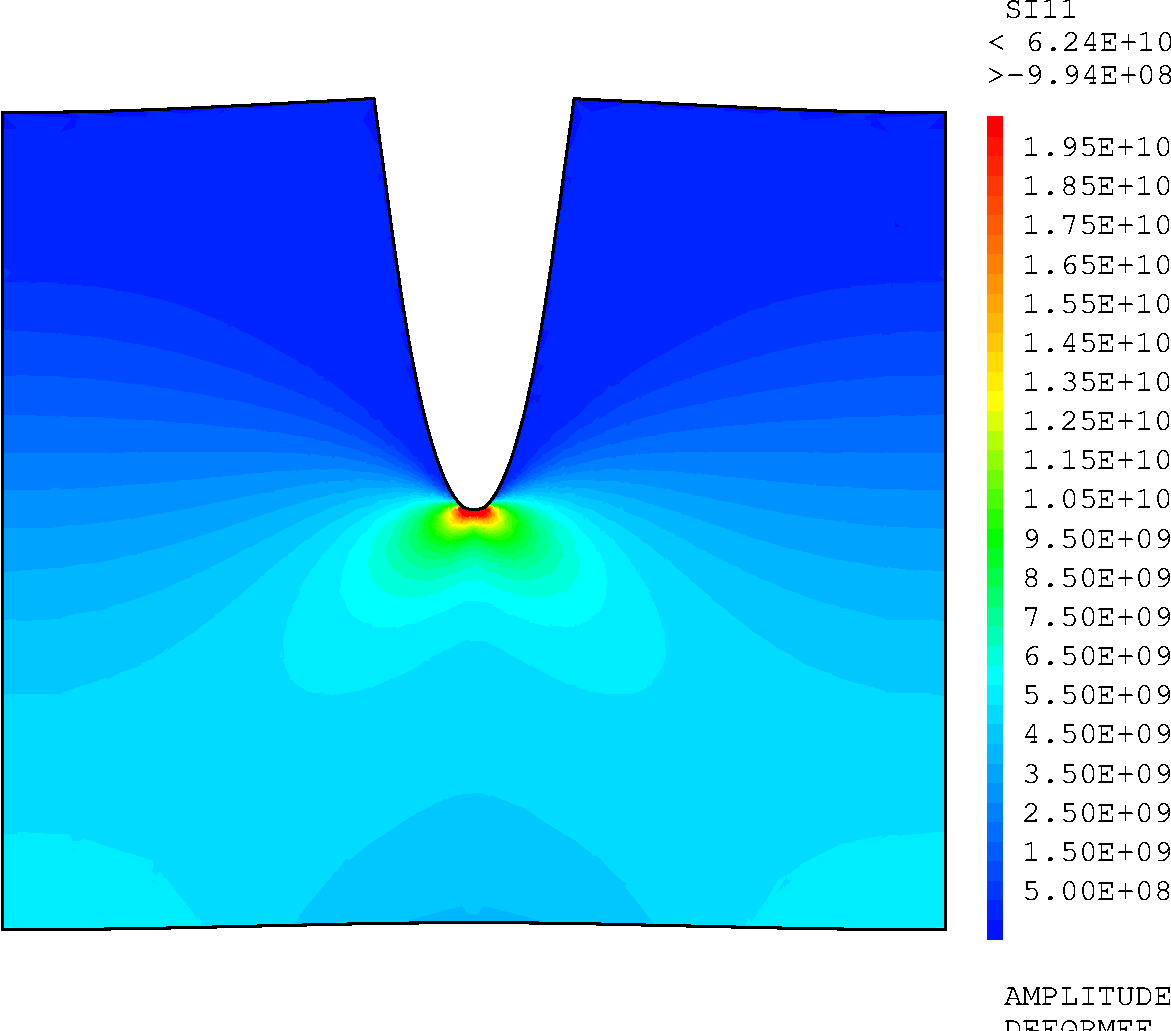
\includegraphics[height=3.5cm]{images/exo/exo_2_sigma.20} \hspace{0.2cm}
    \fi
    \item<2-> \fe{\green{Objectif : \g{supprimer les éléments} au cours du calcul}\\
                  On utilisera un critère de rupture simple sur la 1ère contrainte principale :
                  \begin{center}
                    rupture si $\sigma_I \geq$ 10~GPa\\ \avous{~À vous de jouer !}
                  \end{center}}
                 {\green{Purpose: \g{remove the elements} during calculations}\\
                  We will use a simple fracture criterion based on the 1st principal stress:
                  \begin{center}
                    fracture if $\sigma_I \geq$ 10~GPa\\ \avous{~It's up to you!}
                  \end{center}}
  \end{itemize}
\end{frame}
}

{\setbeamerfont{framesubtitle}{size=\tiny}
\begin{frame}{\fe{Exercice 2 : fissuration par suppression d'éléments}
                 {Exercise 2: fracture by elements removal}}
             {\url{https://www-cast3m.cea.fr/index.php?page=exemples&exemple=formation_pasapas_2_initial}}
  \begin{itemize}
    \item \fe{Quelques opérateurs utiles}{Some useful operators}\\
    \small
    \begin{tabular}{ll}
      \kwr{PRIN} & \fe{pour calculr les contraintes principales}{to compute principal stresses}\\
      \kwr{CHAN} & \fe{pour changer les points support d'un champ}{to change the support points of a field}\\
      \kwr{ELEM} & \fe{pour extraire les éléments d'un champ selon une condition}{to extract the elements of a field that meets a criteria}\\
      \kwr{REDU} & \fe{pour réduire un modèle sur un sous maillage}{to reduce a model on a sub part of a mesh}
    \end{tabular}
    \normalsize
    \item \fe{Quelques indices utiles de la table}{Some useful table indices}\\
    \small
    \begin{tabular}{ll}
      \kwg{ESTIMATION}\kw{.}\kwg{CONTRAINTES}  & \fe{champ de contraintes courant}{current stress field}\\
      \kwg{WTABLE}\kw{.}\kwg{MODELE}           &\fe{modèle courant}{current model}\\
      \kwg{WTABLE}\kw{.}\kwg{CARACTERISTIQUES} & \fe{paramètres matériau courants}{curent material properties}
    \end{tabular}
    \normalsize
  \end{itemize}
\end{frame}
}

\begin{frame}{\fe{Exercice 2 : fissuration par suppression d'éléments}
                 {Exercise 2: fracture by elements removal}}
             {\fe{Solution avec PERSO1}{Solution with PERSO1}}
  \footnotesize
  \begin{itemize}
    \small
    \item \fe{Utiliser la procédure \kwv{PERSO1}}{Use procedure \kwv{PERSO1}}
    \item \fe{Extraire le modèle et les contraintes dans \kwg{ESTIMATION}}{Extract the model and stress field in \kwg{ESTIMATION}}
    \item \fe{Calculer la contrainte principale $\sigma_I$}{Compute the 1st principal stress $\sigma_I$}
    \item \fe{Extraire les éléments "intacts"}{Extract the "intact" elements}
    \item \fe{Réduire le modèle sur ce maillage et écraser \kwg{WTABLE}\kw{.}\kwg{MODELE}}
             {Reduce the model on this mesh and overwrite \kwg{WTABLE}\kw{.}\kwg{MODELE}}
  \end{itemize}
  \vspace{4.5cm}
  \scriptsize
  \begin{textblock*}{10cm}(0.3cm,-4cm)
    \fe{\emph{Programme principal}}{\emph{Main program}}
    \lstinputlisting[basicstyle=\ttfamily\tiny, language=gibiane, firstline=88, lastline=89]{dgibi/formation_pasapas_2_solution.dgibi}
  \end{textblock*}
  \begin{textblock*}{10cm}(5.8cm,-4cm)
    \fe{\emph{\violet{Procédure PERSO1}}}{\emph{\violet{PERSO1 procedure}}}
    \lstinputlisting[basicstyle=\ttfamily\tiny, language=gibiane, firstline=70, lastline=79]{dgibi/formation_pasapas_2_solution.dgibi}
  \end{textblock*}
\end{frame}

\begin{frame}{\fe{Exercice 2 : fissuration par suppression d'éléments}
                 {Exercise 2: fracture by elements removal}}
             {\fe{Solution avec PERSO1}{Solution with PERSO1}}
  \footnotesize
  \begin{itemize}
    \item \fe{Résultats}{Results}\\
    \hspace{3cm}
    \if \animation 1
      \animategraphics[controls,loop,poster=last,height=4.5cm]{7}{images/exo/exo_2_solu_sigma.}{01}{20} \hspace{1.5cm}
    \else
      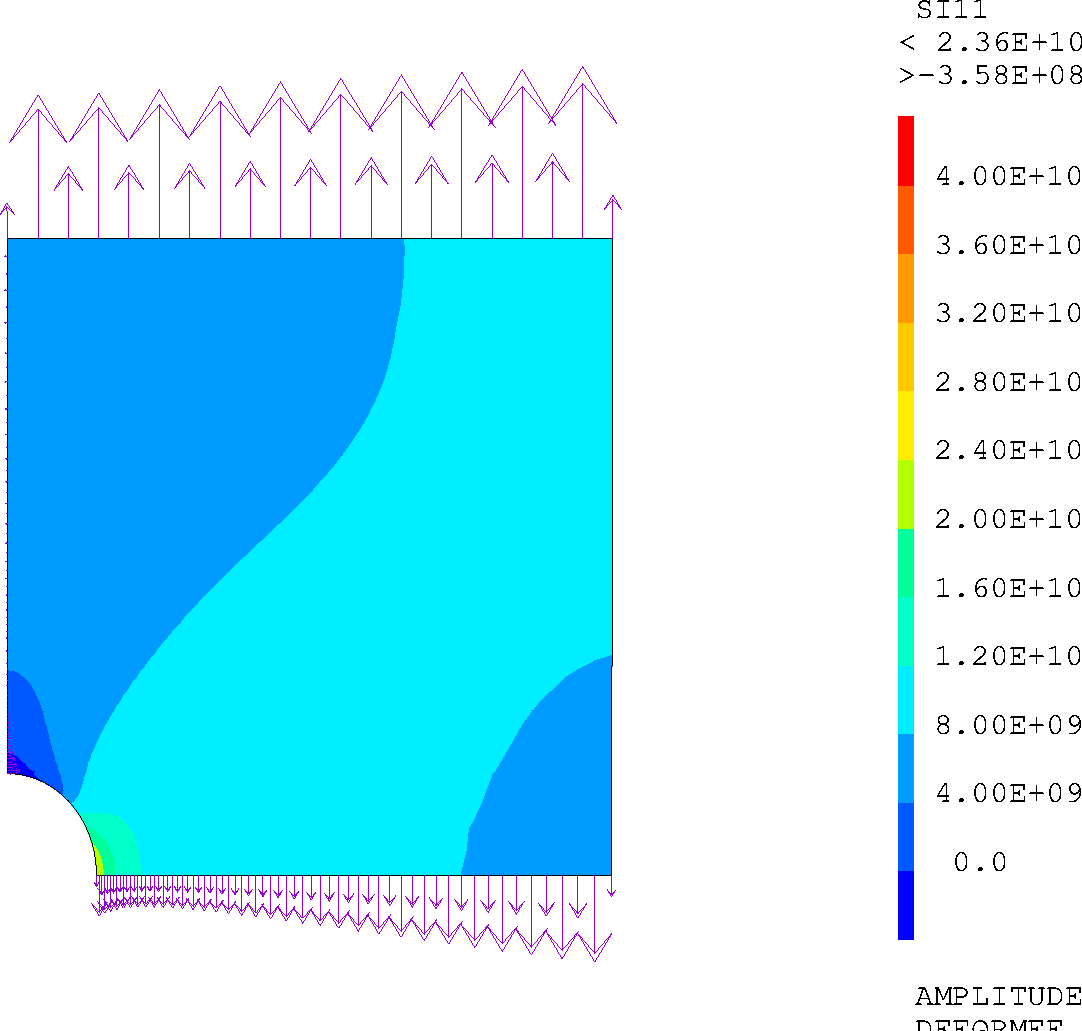
\includegraphics[height=4.5cm]{images/exo/exo_2_solu_sigma.20} \hspace{1.5cm}
    \fi
    \item \fe{Modèle peu robuste\\ résultats très sensibles à la discrétisation espace/temps}
             {Undependable model\\ results quite sensitive to time/space discretization}
  \end{itemize}
\end{frame}
